% Beamer slide template prepared by Tom Clark <tom.clark@op.ac.nz>
% Otago Polytechnic
% Dec 2012

\documentclass[10pt]{beamer}
\usetheme{Dunedin}
\usepackage{graphicx}
\usepackage{fancyvrb}

\newcommand\codeHighlight[1]{\textcolor[rgb]{1,0,0}{\textbf{#1}}}

\title{Puppet Introduction}

\author[IN719]{Systems Administration}
\institute[Otago Polytechnic]{
  Otago Polytechnic \\
  Dunedin, New Zealand \\
}
\date{}
\begin{document}

%----------- titlepage ----------------------------------------------%
\begin{frame}[plain]
  \titlepage
\end{frame}

%----------- slide --------------------------------------------------%
\begin{frame}
  \frametitle{The problem}

 \begin{itemize}
  \item Configuring systems one at a time is too slow.
  \item One at a time configuration can lead to inconsistencies.
  \item Information about how your systems are configured winds up scattered across your network.
  \end{itemize}



\end{frame}

%----------- slide --------------------------------------------------%
\begin{frame}
  \frametitle{The solution: configuration management systems}

  We'll store all of the configuration information on a central server that will push configurations out to 
  client machines.  This will
  
  \begin{itemize}
  \item Get all of our configuration information in one place.
  \item Ensure that configuration is consistently and promptly applied to all systems.
  \item Save time!
  \end{itemize}

\end{frame}

%----------- slide --------------------------------------------------%
\begin{frame}
  \frametitle{Examples of configuration management systems}

  In this paper we will use \emph{Puppet} for configuration management.
  
  \begin{itemize}
  \item Ansible
  \item Chef
  \item Puppet
  \item Salt
  \end{itemize}

\end{frame}


%----------- slide --------------------------------------------------%
\begin{frame}
  \frametitle{Puppet}

  In this paper we will use \emph{Puppet} for configuration management.
  
  \begin{itemize}
  \item It is mature and powerful.
  \item It is widely used.
  \item It is reasonably cross-platform.
  \end{itemize}

\end{frame}

%----------- slide --------------------------------------------------%
\begin{frame}
  \frametitle{Puppet overview}

  Our \texttt{mgmt} servers will manage Puppet for us.  In Puppet terms, these servers will be \emph{puppetmasters}.
  
  The client machines (including the \texttt{mgmt} servers) will be \emph{agents}.  They periodically contact the puppetmaster to get new configuration information.
  
\end{frame}
%----------- slide --------------------------------------------------%
\begin{frame}[fragile]
  \frametitle{Puppet overview}

  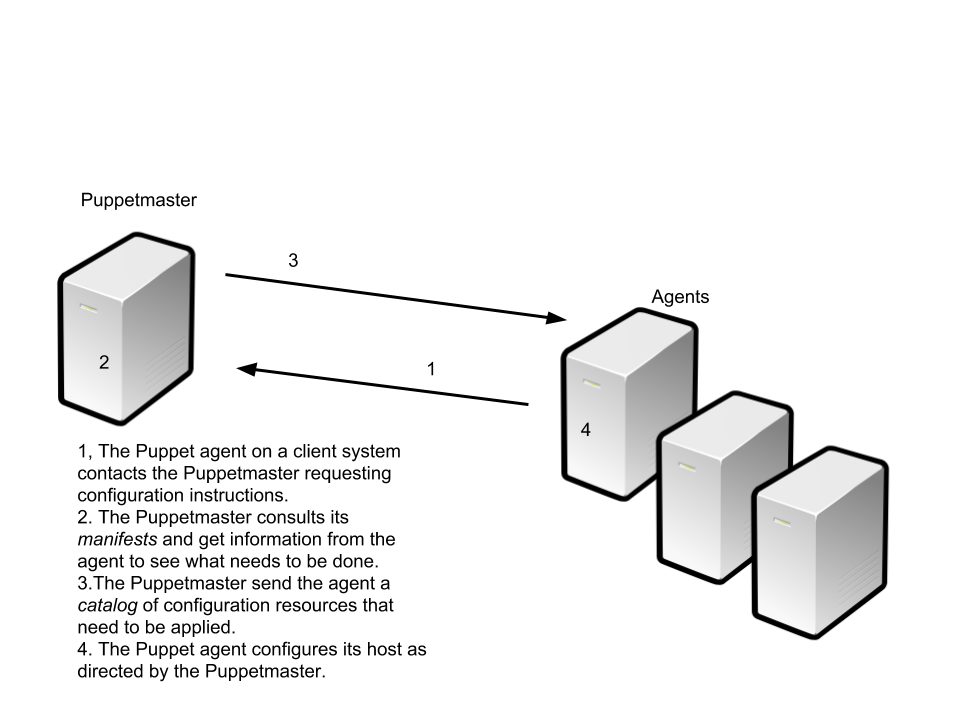
\includegraphics[width=90mm]{puppet.png} 
   
\end{frame}
%----------- slide --------------------------------------------------%
\begin{frame}
  \frametitle{Some Key Terms}

 \begin{description}
  \item[Manifest] Any bit of Puppet code stored in a file that ends with the .pp extension.  These sit on the puppetmaster.
  \item[Node] A collection of resources in a manifest that will be applied to a particular agent.
  \item[Catalog] The puppetmaster reads the manifests and compiles a catalog for each host. A catalog is a set of resources to be used on an agent system.
  \item[Resource]A unit of puppet configuration.  A resources has a \emph{type}, a \emph{title}, and one or more \emph{attributes}.

  \end{description}

\end{frame}
%----------- slide --------------------------------------------------%
\begin{frame}
  \frametitle{Some Types}

Puppet supports many standard types, and it is possible to define your own.  Some important types include:
\begin{itemize}
\item Package
\item File
\item Service
\item User
\item Group
\item Exec
\item Cron
\end{itemize}


\end{frame}

%----------- slide --------------------------------------------------%
\begin{frame}[fragile]
  \frametitle{Nodes}

A node is basically a host you want to configure.
\begin{verbatim}
node 'www.foo.org.nz' {

}

node 'db1.foo.org.nz', 'db2.foo.org.nz' {

}
\end{verbatim}


\end{frame}

%----------- slide --------------------------------------------------%
\begin{frame}[fragile]
  \frametitle{The Default Node}

If you specify a \emph{default} node, its configuration will be applied to any node that does not have a specific node definition.
\begin{verbatim}
node default {

}
\end{verbatim}


\end{frame}

%----------- slide --------------------------------------------------%
\begin{frame}[fragile]
  \frametitle{Node Inheritance}

A node can inherit from another node.  For example 'www.foo.org.nz' gets all of the configuration from the base node, plus it's own specific configuration.

\begin{verbatim}
node base {

}

node 'www.foo.org.nz' inherits base {

}
\end{verbatim}

Note that Puppet best practice is to be careful to avoid overusing inheritance.  If you find yourself going back and modifying base classes or adding and removing inheritance relationships often, that is a sign that you shouldn't be using inheritance.

\end{frame}
%----------- slide --------------------------------------------------%
\begin{frame}[fragile]
  \frametitle{Applying Configuration to a Node}



\begin{verbatim}
node 'db.foo.org.nz' {
  packaage { 'vim':
             ensure => installed,
           }  
              
}
\end{verbatim}


\end{frame}


%----------- slide --------------------------------------------------%
\begin{frame}[fragile]
  \frametitle{Modules}
  A collection of related resources can be organised into a \emph{module}.  For example, we may want to install the nginx package, its configuration file, and set up a document root directory.  We can create a module that incorporates all of these things, and then use the module in a node:

\begin{verbatim}
node 'app.foo.org.nz' {
  include nginx-webserver
}
\end{verbatim}

We will create and apply a module in today's lab.



\end{frame}

\end{document}
